\chapter{Class F Amplifier ADS Simulations, Comparisons to Specs}

The initial goal of the class F amplifier design was to try and control up the fifth harmonic which would ideally allow 90.5\% drain efficiency and to have a center frequency of 5 GHz. After looking through the past amplifier competitions and looking at various RF transistor manufacturers, the Wolfspeed CGHV1F006S GaN HEMT transistor was chosen. This model was chosen over others to the relatively new release of the transistor, the high operating frequency of the transistor (18 GHz), and the fact that the transistor came in a QFP package versus a semiconductor die. The majority of past winners of the amplifier competition used Cree (now Wolfspeed) transistors and Wolfspeed provides a transistor level models for the amplifier for accurate simulations to design amplifiers. The design goals are in Table \ref{table:design_goal}, the initial goals were relatively aggressive in trying to push the PAE and center frequency for the highest figure of merit. After simulating, fabricating, and testing multiple versions the design goals were set to a more conservative value. This chapter discusses the simulations results of the final version of the amplifier.

The initial design was pushing the limits of the specification by attempting to achieve the minimum output power with the highest allowed input power. This was risky because designing for the minimum gain allows for little margin for non-ideal factors that couldn't be taken into account of the simulation. The first amplifier that I fabricated had a simulated gain of X with a PAE of Y at an input power of Z dBm. The amplifier initially had a short from the drain and explain more. Once the amplifier was working the measured gain was only A so even at the maximum allowed input power of 24 dBm, it would not be able to deliver 36 dBm of power. For the final version of the amplifier, the design margins were increased substantially so stuff could happen better.

%REWORK

\begin{table}
    \centering
    \caption{Design Goals of Amplifier}
    \label{table:design_goal}
    \begin{tabular}{|l|l|l|}
      \hline
      % after \\: \hline or \cline{col1-col2} \cline{col3-col4} ...
      {Parameter} & {Initial Goal}     & {Final Goal} \\ \hline
      {Center Frequency, GHz} & 5    & 3 \\ \hline
      {PAE, \%}               & 80 & 70 \\ \hline
      {Gain, dB}              & 15 & 22 \\ \hline
    \end{tabular}
\end{table}

\section{DC Bias Point}
The simulation of the various parts of the class F amplifier was done using Keysight ADS 2016. The first step in the simulation process was determining the optimal DC bias. Using the provided transistor model from Wolfspeed, various drain and gate voltages were simulated to see what the drain current and transducer gain CHECK THIS STATEMENT the transistor would have using the circuit seen in Figure \ref{fig:bias_ckt}. The bias for the class F amplifier should be in the "deep" AB region so the drain current resembles a half sinusoid shape but still allows for the negative third harmonic to be present. The drain current should be minimized in order to maximize the PAE of the amplifier. The competition rule states the amplifier should have a minimum of 36 dBm output power at a maximum of 24 dBm input power resulting in a minimum gain of 12 dBm. For the final amplifier, the target gain was 22 dB so there would be a margin for various effects that wouldn't be able to be taken into account in the simulation like the fabrication process. The transistor maximum operating ratings can be seen in Table \ref{table:trans_param}.

\begin{table}
    \centering
    \caption{Maximum Operating Parameters of CGHV1F006S Transistor}
    \label{table:trans_param}
    \begin{tabular}{|l|l|}
      \hline
      % after \\: \hline or \cline{col1-col2} \cline{col3-col4} ...
      {Parameter} & {Rating}\\ \hline
      {Maximum Drain-Source Voltage, V} & 100 \\ \hline
      {Maximum Drain-Source Current, A} & 0.95\\ \hline
      {Maximum Gate-Source Voltage, V}  & -10,+2 \\ \hline
      {Maximum Gate-Source Current, mA} & 1.2 \\ \hline
    \end{tabular}
\end{table}

A starting point to select the gate voltage is to choose a value so the drain current is 10\% of the maximum current so the conduction cycle is close to $\pi$. The final version of the amplifier had a gate source voltage of -2.4 V which in Figure (Ids vs Vds) figure is in the "deep AB" region of the device as shown in Figure \ref{fig:ids_versus_vds} and draws only 80 mA of quiescent current. The drain-source voltage was chosen to be 40 V because it's the recommended operating voltage from the datasheet for the transistor. After the gate voltage was selected, the stability factor ($k$) and the stability measurement ($\Delta$) were then simulated to see what the stability of the amplifier is near the center frequency seen in Figures \ref{fig:stab_fact} and \ref{fig:stab_meas} respectively. For an amplifier to be unconditionally stable, $k$ must be greater than one and $\Delta$ be positive CITE NEEDED, and because $k$ is less than one the amplifier has potentially unstable regions. The stability regions of the load and source plane were then simulated to determine a starting point for the load and source pulls. The results of the load and source stability regions can be seen in Figures \ref{fig:load_stab} and \ref{fig:source_stab}. The region of stability for both stability circles is outside the circle.

%Plot of bias circuit

\begin{figure}
  \centering
  % Requires \usepackage{graphicx}
  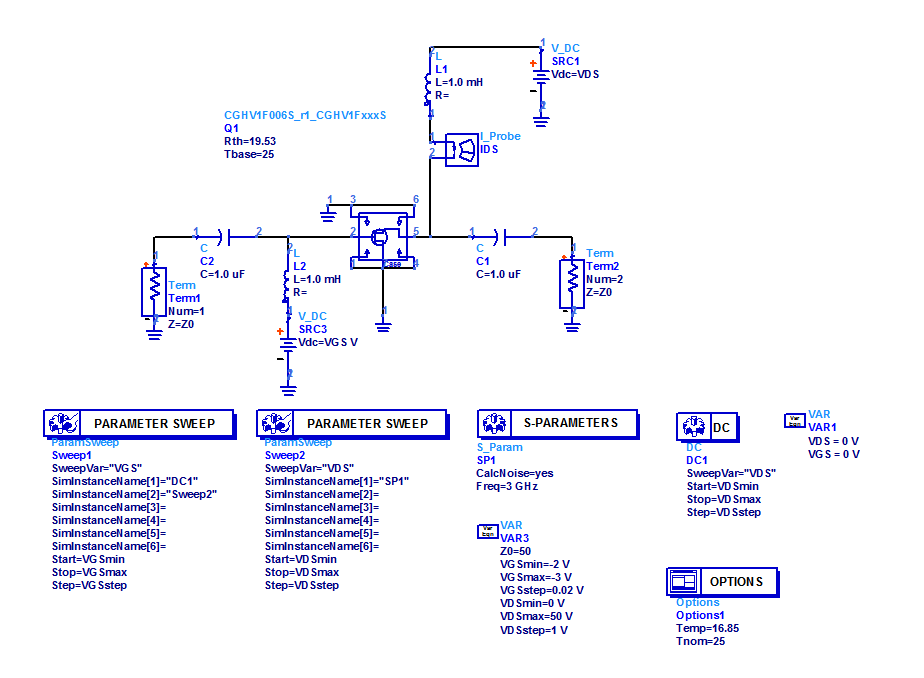
\includegraphics[width=6in,height=6in,keepaspectratio]{figures/simulation/bias_ckt}\\
  \caption{Bias Circuit Setup}
  \label{fig:bias_ckt}
\end{figure}

%Plot of Ids vs Vds and maximum transducer gain
\begin{figure}
  \centering
  % Requires \usepackage{graphicx}
  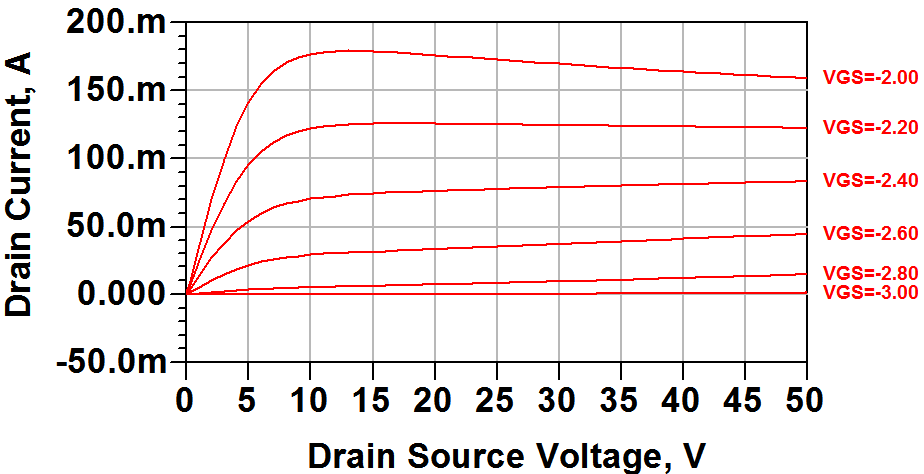
\includegraphics[width=5in,height=5in,keepaspectratio]{figures/simulation/ids_versus_vds}\\
  \caption{Drain Current versus Drain Voltage for Various Gate Voltages}
  \label{fig:ids_versus_vds}
\end{figure}

\begin{figure}
  \centering
  % Requires \usepackage{graphicx}
  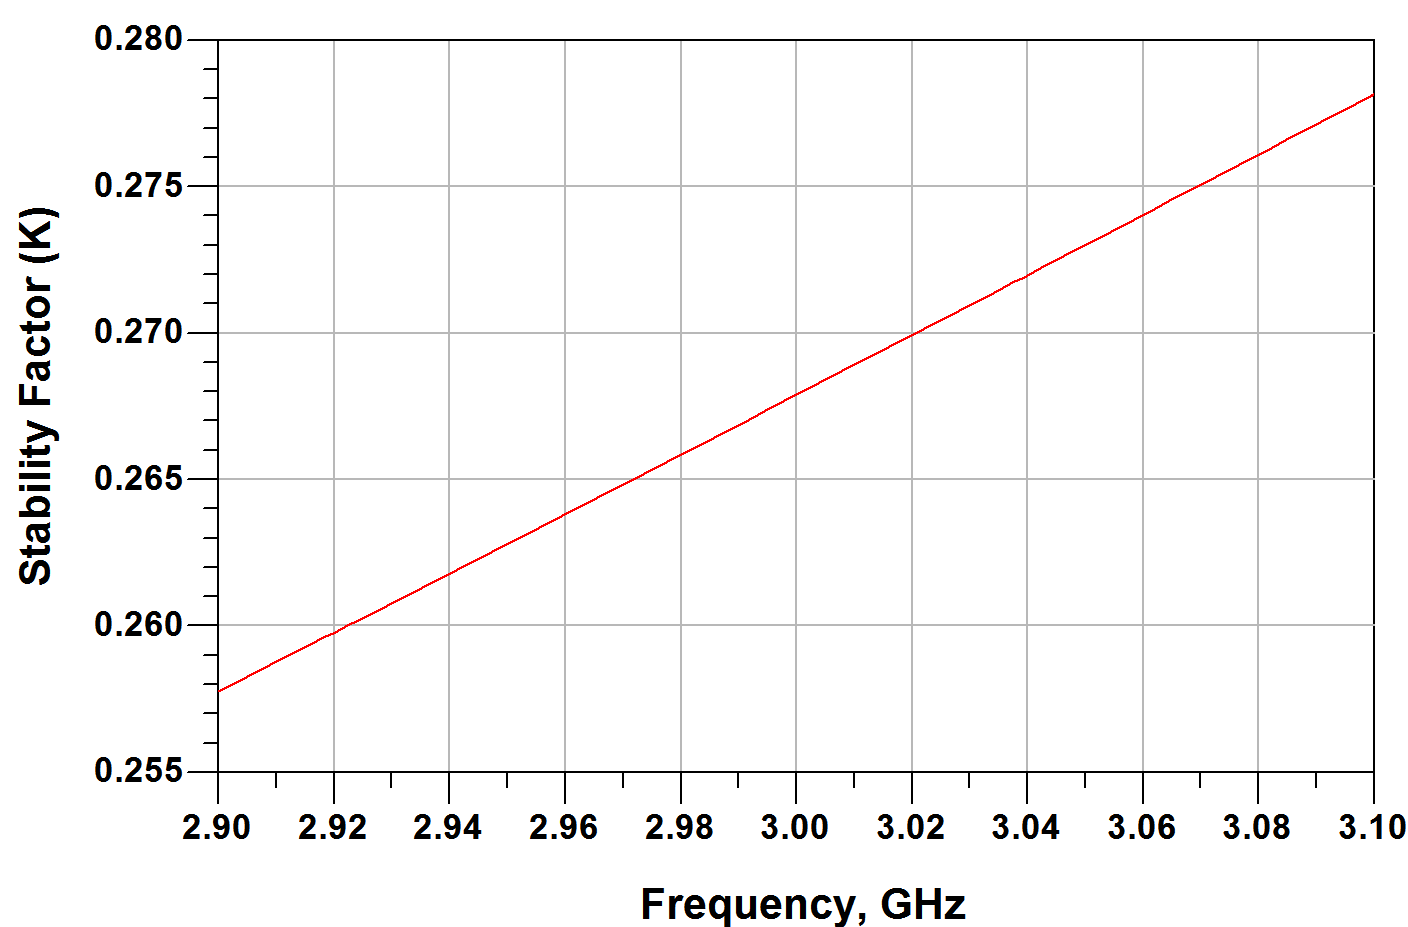
\includegraphics[width=5in,height=5in,keepaspectratio]{figures/simulation/stab_fact}\\
  \caption{Stability Factor ($k$) versus Frequency}
  \label{fig:stab_fact}

  \vspace*{\floatsep}

  \centering
  % Requires \usepackage{graphicx}
  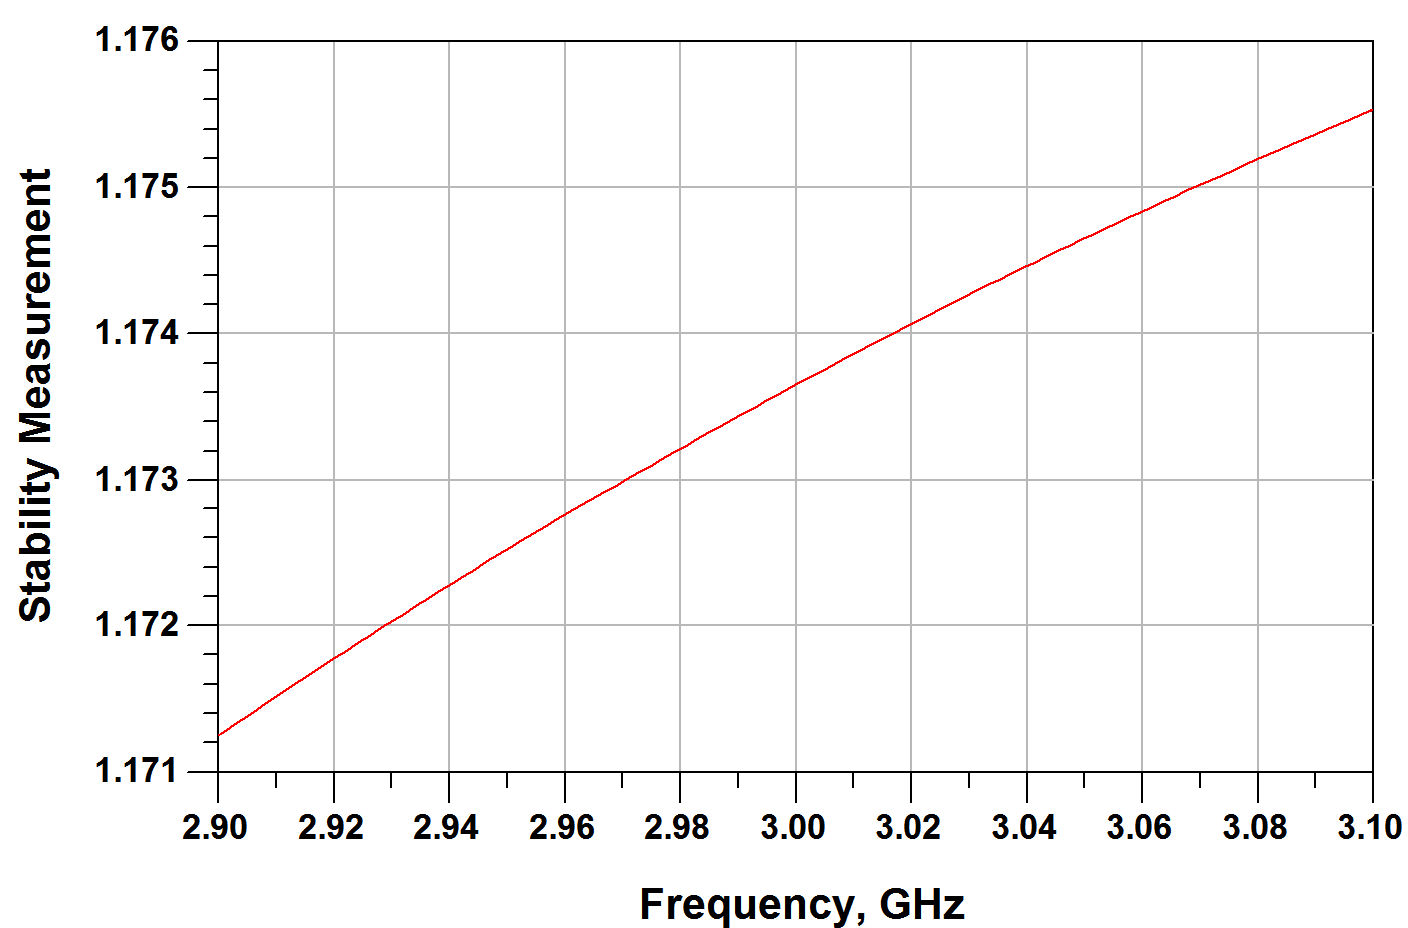
\includegraphics[width=5in,height=5in,keepaspectratio]{figures/simulation/stab_meas}\\
  \caption{Stability Measure ($\Delta$) versus Frequency}
  \label{fig:stab_meas}
\end{figure}

\begin{figure}
  \centering
  % Requires \usepackage{graphicx}
  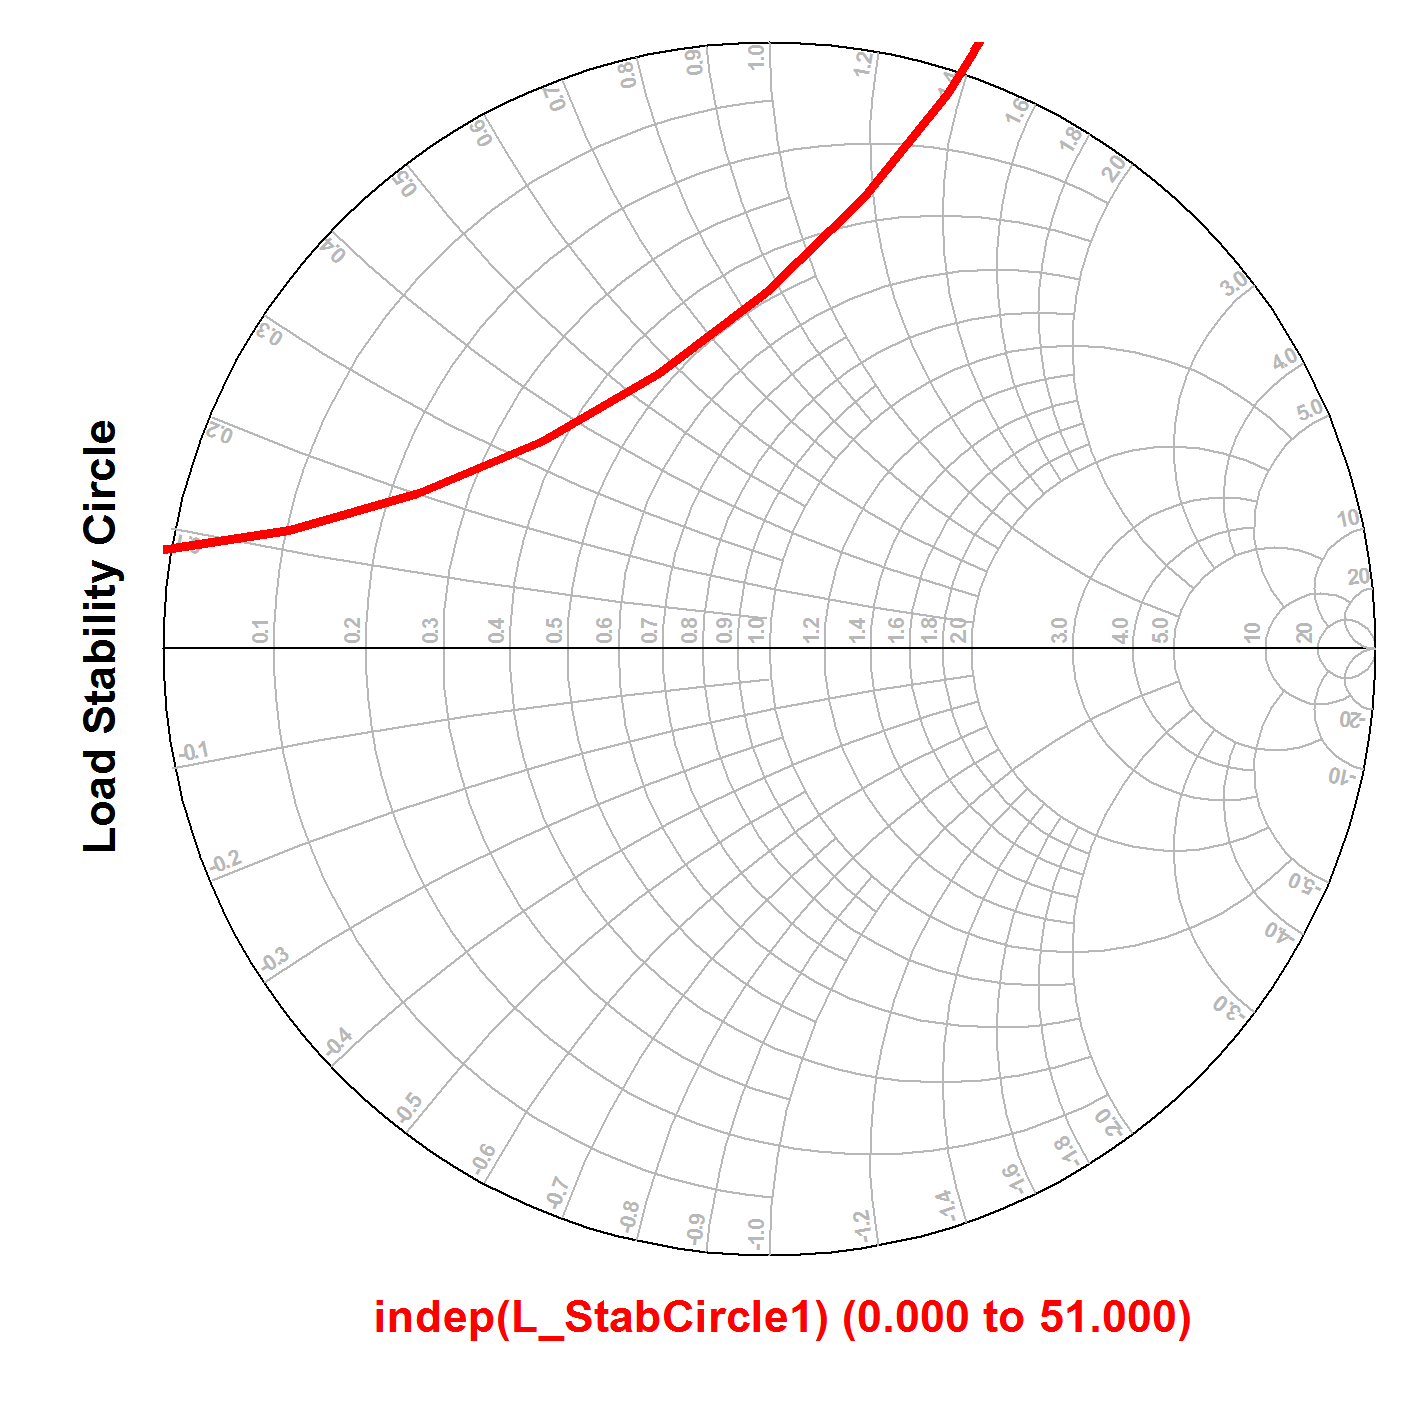
\includegraphics[width=4in,height=4in,keepaspectratio]{figures/simulation/load_stab}\\
  \caption{Load Stability Circle of Transistor. Stable Region Outside of Circle}
  \label{fig:load_stab}

  \vspace*{\floatsep}

  \centering
  % Requires \usepackage{graphicx}
  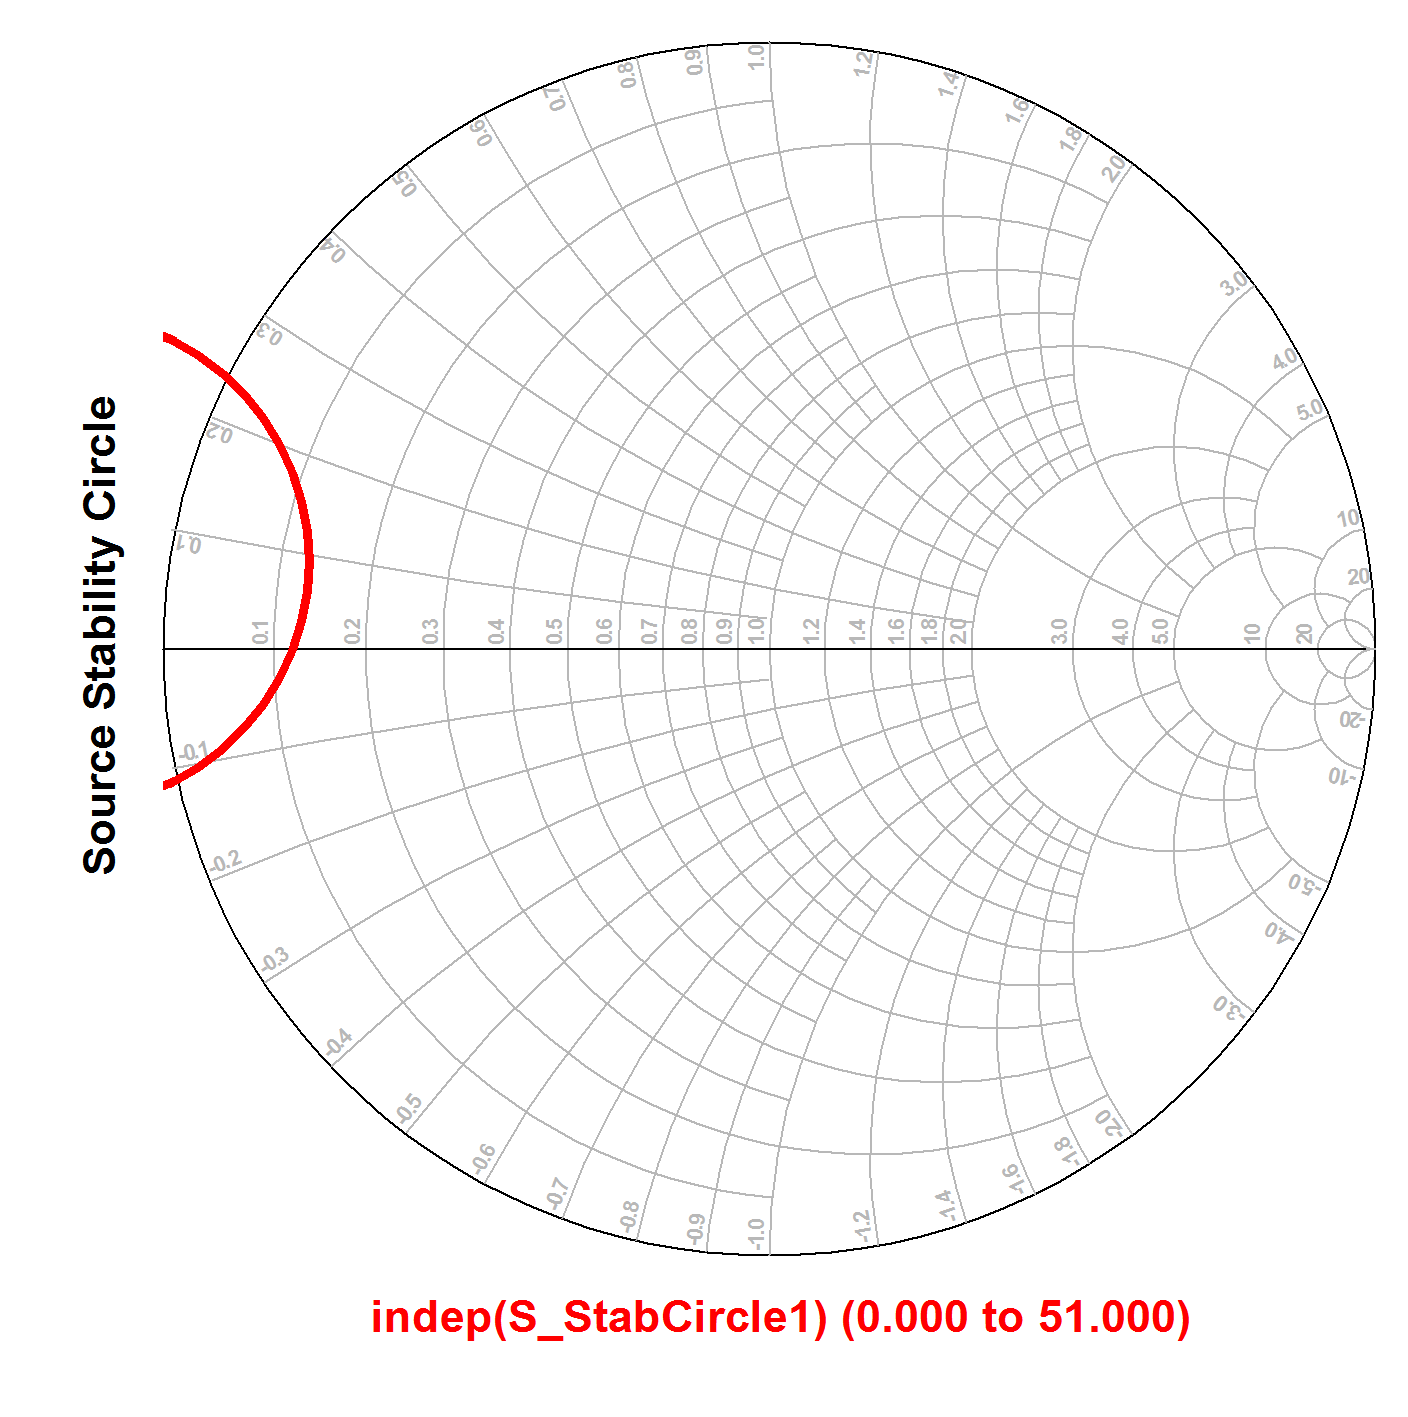
\includegraphics[width=4in,height=4in,keepaspectratio]{figures/simulation/source_stab}\\
  \caption{Source Stability Circle of Transistor. Stable Region Outside of Circle}
  \label{fig:source_stab}
\end{figure}



%Talk about simulation results

\section{Talk about fundamental load and source pull}

After determining the DC bias of the amplifier, fundamental load and source pulls are done to determine the optimal load and source impedances for the transistor. Load pulls are done keeping the source impedance fixed and sweeping the load over a uniformly sampled space on the Smith Chart to then measuring the transducer gain. Various drain efficiency and gain contours can be produced by doing load pulls. The typical process starts with sampling the entire Smith Chart then load pulling again around the region with the highest efficiency contour. As a starting point the source impedance was set to a low impedance of 10$\Omega$ but still outside of the source stability circle. Source pulling is done after load pulling and follows a similar process by keeping the load impedance fixed then sweeping the source impedance for the highest efficiency while still having the target gain. The load and source pulls are done at the fundamental frequency at an input power of 15 dBm to provide an additional margin in the design. In practice the amplifier the amplifier will require a higher input power to achieve the simulation results due to losses that could not be simulated in ADS FLESH OUT. Also the source and load impedances for the higher harmonics are shorted.

For the sake of brevity only the final load and source pull results are shown but the process will be described. The initial load pull results showing PAE and power delivered contours can be seen in Figure \ref{fig:smith_fund_load} and \ref{fig:xy_fund_load}. The highest power delivered is only 35.45 dBm at a drain efficiency of 35\% while the highest PAE 40\% results in a power delivered of 35.2 dBm. The PAE should be less than 50\% because an amplifier with only the fundamental present is a class A amplifier with a maximum efficiency of 50\%. As more harmonics are properly added the power delivered and PAE should increase. The final fundamental load impedance selected from the simulation results was 14.3+j54 $\Omega$.

%REWORK next section talks about the final results

%Plots of load pull with efficiency and gain contours
\begin{figure}
  \centering
  % Requires \usepackage{graphicx}
  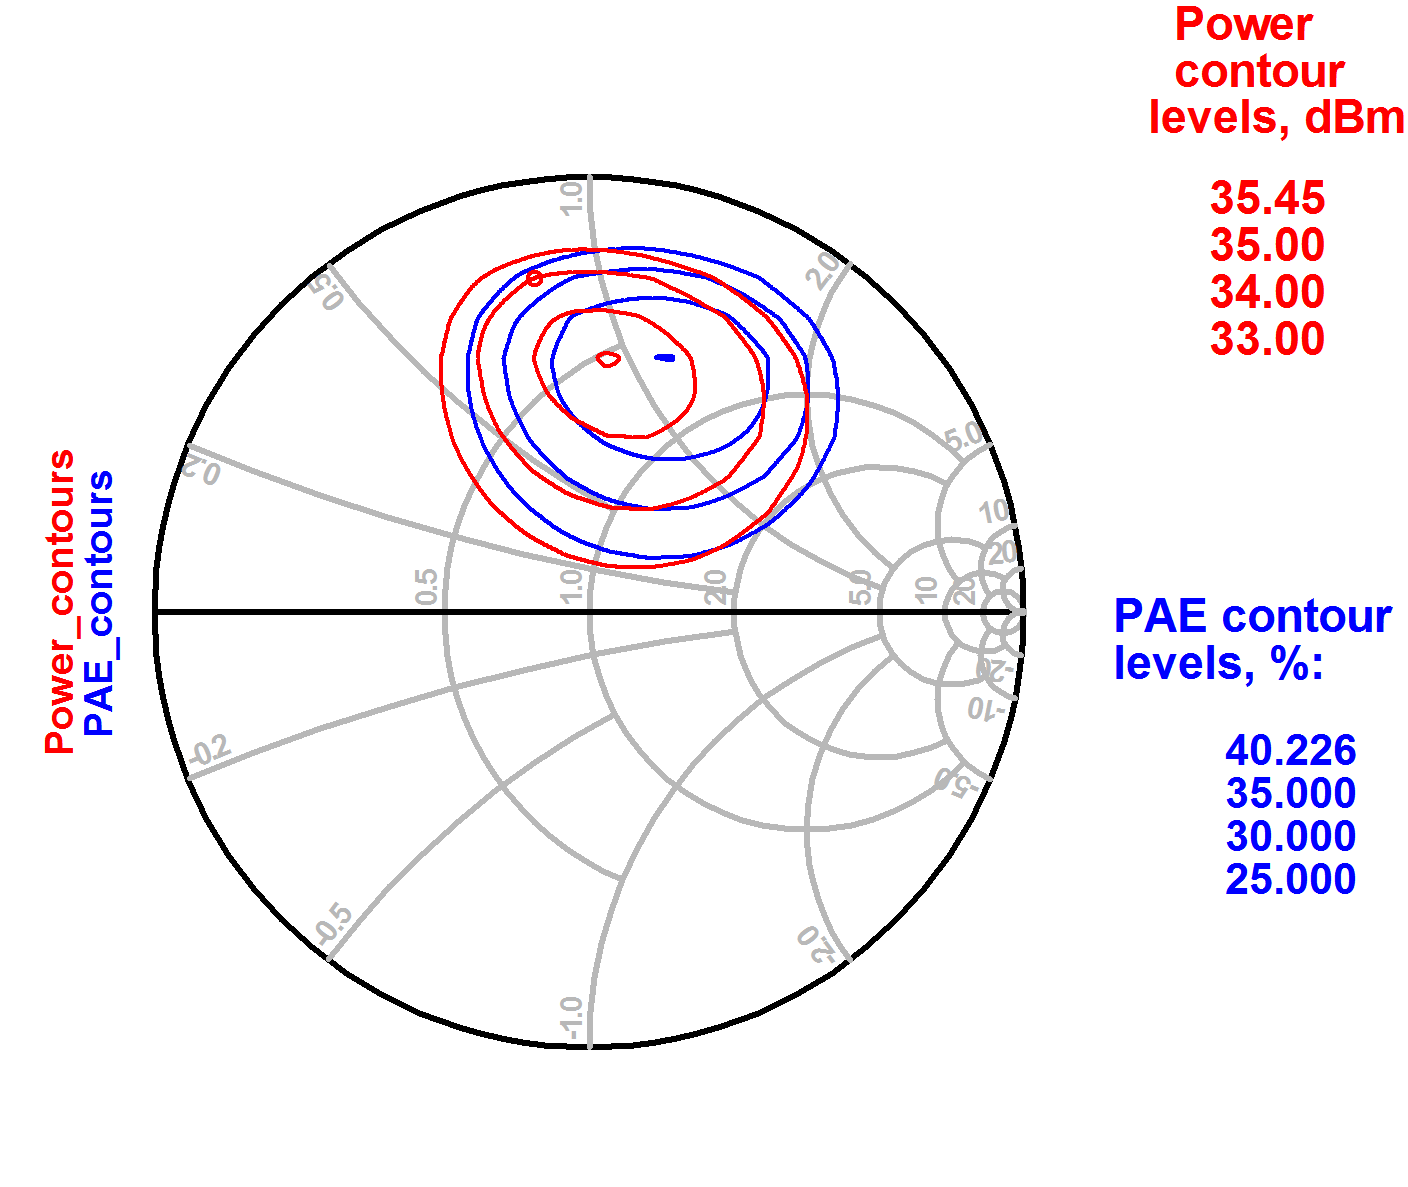
\includegraphics[width=4in,height=4in,keepaspectratio]{figures/simulation/pae_pout_smith_cont_fund}\\
  \caption{Smith Chart Load Pull Simulation Results at 3 GHz with PAE and Power Delivered Contours}
  \label{fig:smith_fund_load}
  
  \vspace*{\floatsep}
  
  \centering
  % Requires \usepackage{graphicx}
  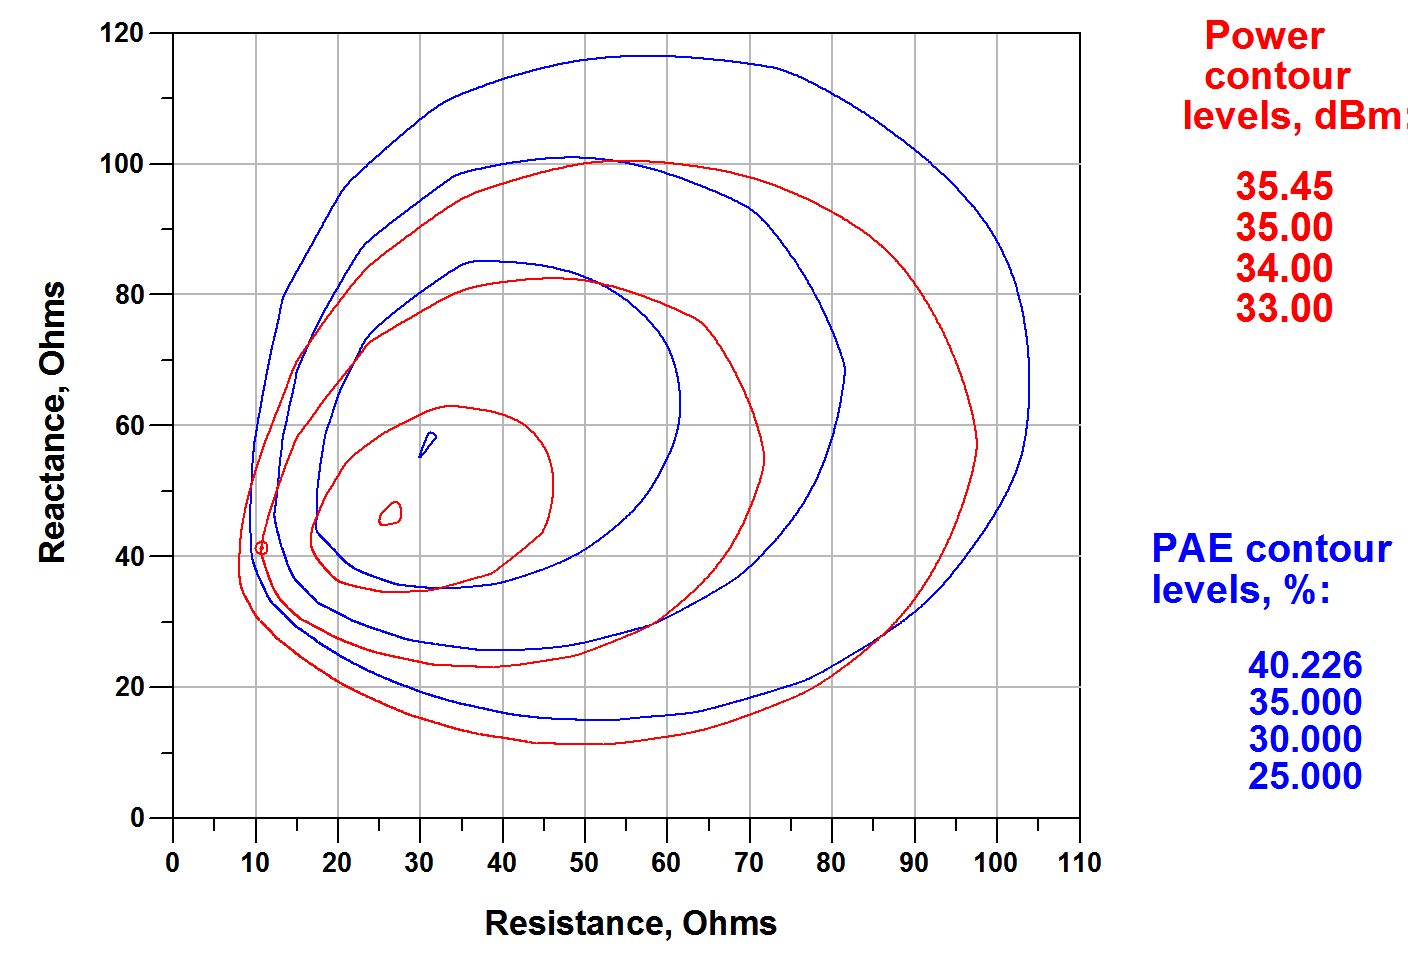
\includegraphics[width=4in,height=4in,keepaspectratio]{figures/simulation/pae_pout_res_cont_fund}\\
  \caption{Don't know how to title this}
  \label{fig:xy_fund_load}
\end{figure}

%Plots of source pull with same as above

The next step is the source pull done with the load set to the impedance discussed earlier. The results of the source pull can be seen in Figures \ref{fig:smith_fund_source} and \ref{fig:xy_fund_source}. The maximum PAE and power delivered has dropped but this isn't unexpected. The pulling process is iterative and if another load pull was done using a new source impedance, one would see the PAE and power delivered increase from the first load pull. Multiple iterations are required to fine tune the parameters because they are dependent on one another. A fundamental source impedance of 3+j3 $\Omega$ was chosen for the final amplifier configuration as a compromise between high PAE while still delivering over 36 dBm of power.

\begin{figure}
  \centering
  % Requires \usepackage{graphicx}
  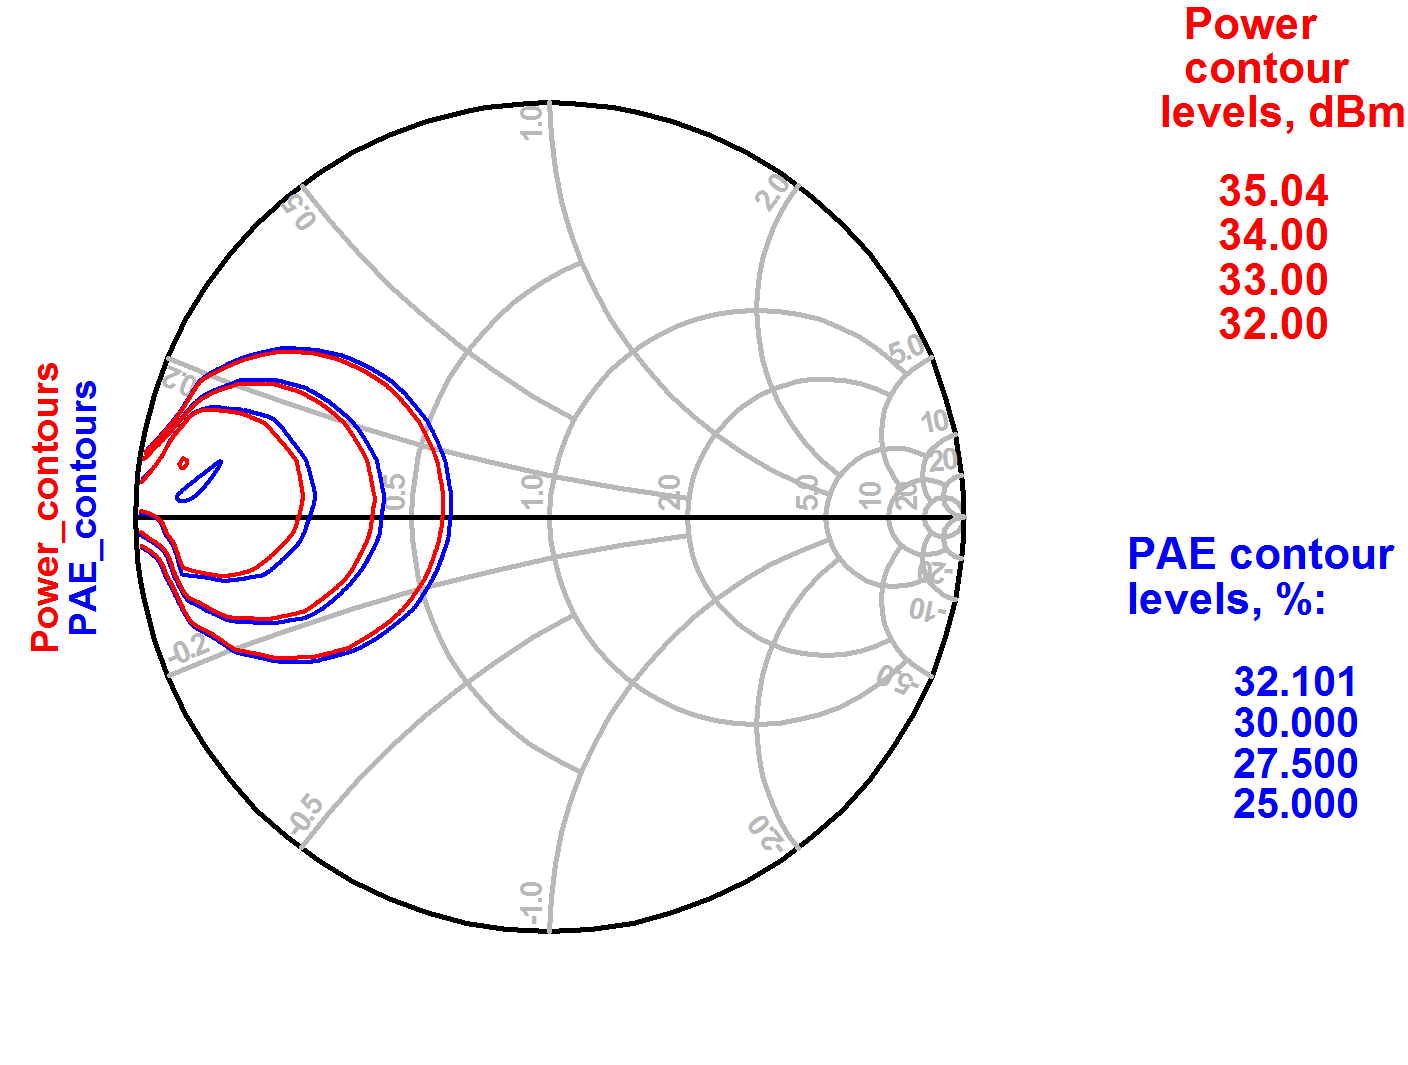
\includegraphics[width=4in,height=4in,keepaspectratio]{figures/simulation/smith_fund_source}\\
  \caption{Smith Chart Source Pull Simulation Results at 3 GHz with PAE and Power Delivered Contours}
  \label{fig:smith_fund_source}

  \vspace*{\floatsep}

  \centering
  % Requires \usepackage{graphicx}
  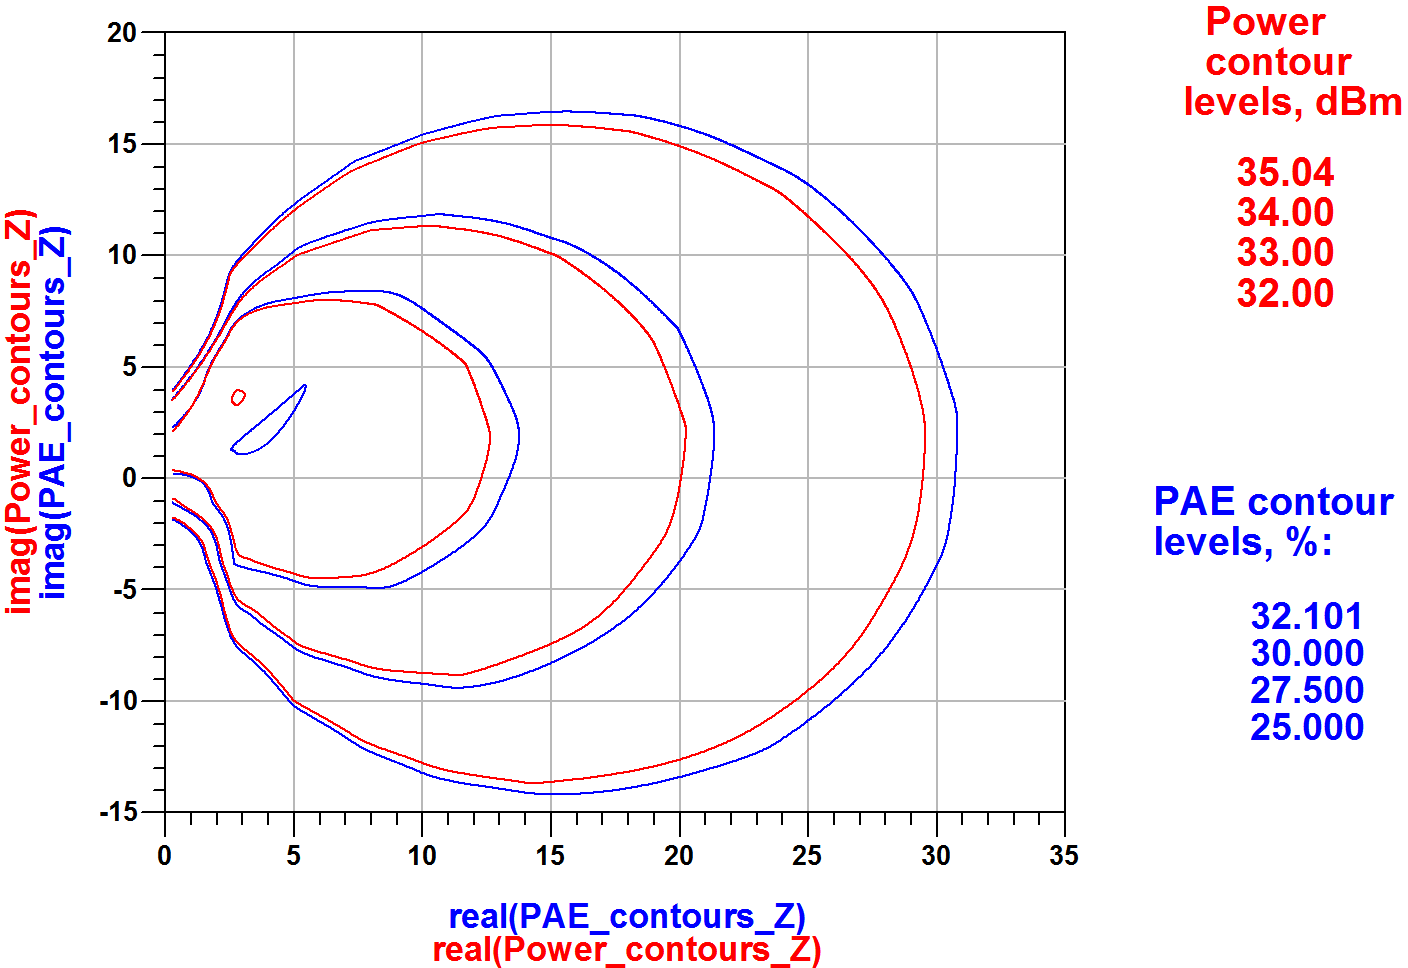
\includegraphics[width=4in,height=4in,keepaspectratio]{figures/simulation/res_fund_source}\\
  \caption{Don't know how to title this}
  \label{fig:xy_fund_source}
\end{figure}

%Talk about simulation results

\section{Harmonic Pulls}

The load and source pulls are done at the fundamental frequency while the harmonic pulls are done at the higher harmonics. The process starts with the second harmonic load pull with the fundamental load and source impedances set to the values determined in the previous section. The source impedance at the second harmonic and all the higher harmonic impedances are set to 0 $\Omega$. After determining the optimal load for maximum PAE while still delivering enough output power, a source pull is done at the second harmonic with the optimal load. This process is then repeated for at the third harmonic. After all of the load and source pulls, one last load pull is done at the fundamental to confirm an the increase of PAE and power delivered. The final fundamental load pull can be seen in Figure \ref{fig:sc_fund_final_load} and \ref{fig:res_cont_fund_load_final}. At the highest power delivered of 38.9 dBm the PAE is 69\% while at the highest PAE of 79\% the output delivered is 36.9 dBm.

A table of the load and source impedances used for the final amplifier configuration can be seen in Table \ref{table:harmonic_impedance}. The final amplifier had an output power of 37 dBm with 22 dB of gain and a PAE of 79.25\% resulting in a figure of merit of 104. While the figure of merit is not the highest compared to the past winners, it is still competitive. The drain efficiency of the final amplifier is 79.2\% which is close to the theoretical maximum of 81.7\%. The source and load impedances are used to design matching networks, this sentence is terrible. The simulated harmonic pulls are used to determine the maximum theoretical performance that can be extracted from the transistor.

\begin{table}
    \centering
    \caption{Final Harmonic Impedances for Amplifier}
    \label{table:harmonic_impedance}
    \begin{tabular}{|l|l|l|} \hline
    % after \\: \hline or \cline{col1-col2} \cline{col3-col4} ...
    {Frequency, GHz} & {Load Impedance, $\Omega$} & {Source Impedance, $\Omega$} \\ \hline
    {3} & {14.3+j54.0} & {3+j3} \\ \hline
    {6} & {1.4+j37.0} & {3-j55} \\ \hline
    {9} & {0.3+j13.4} & {0.5-j2.6} \\ \hline
    \end{tabular}
\end{table}

\begin{figure}
  \centering
  % Requires \usepackage{graphicx}
  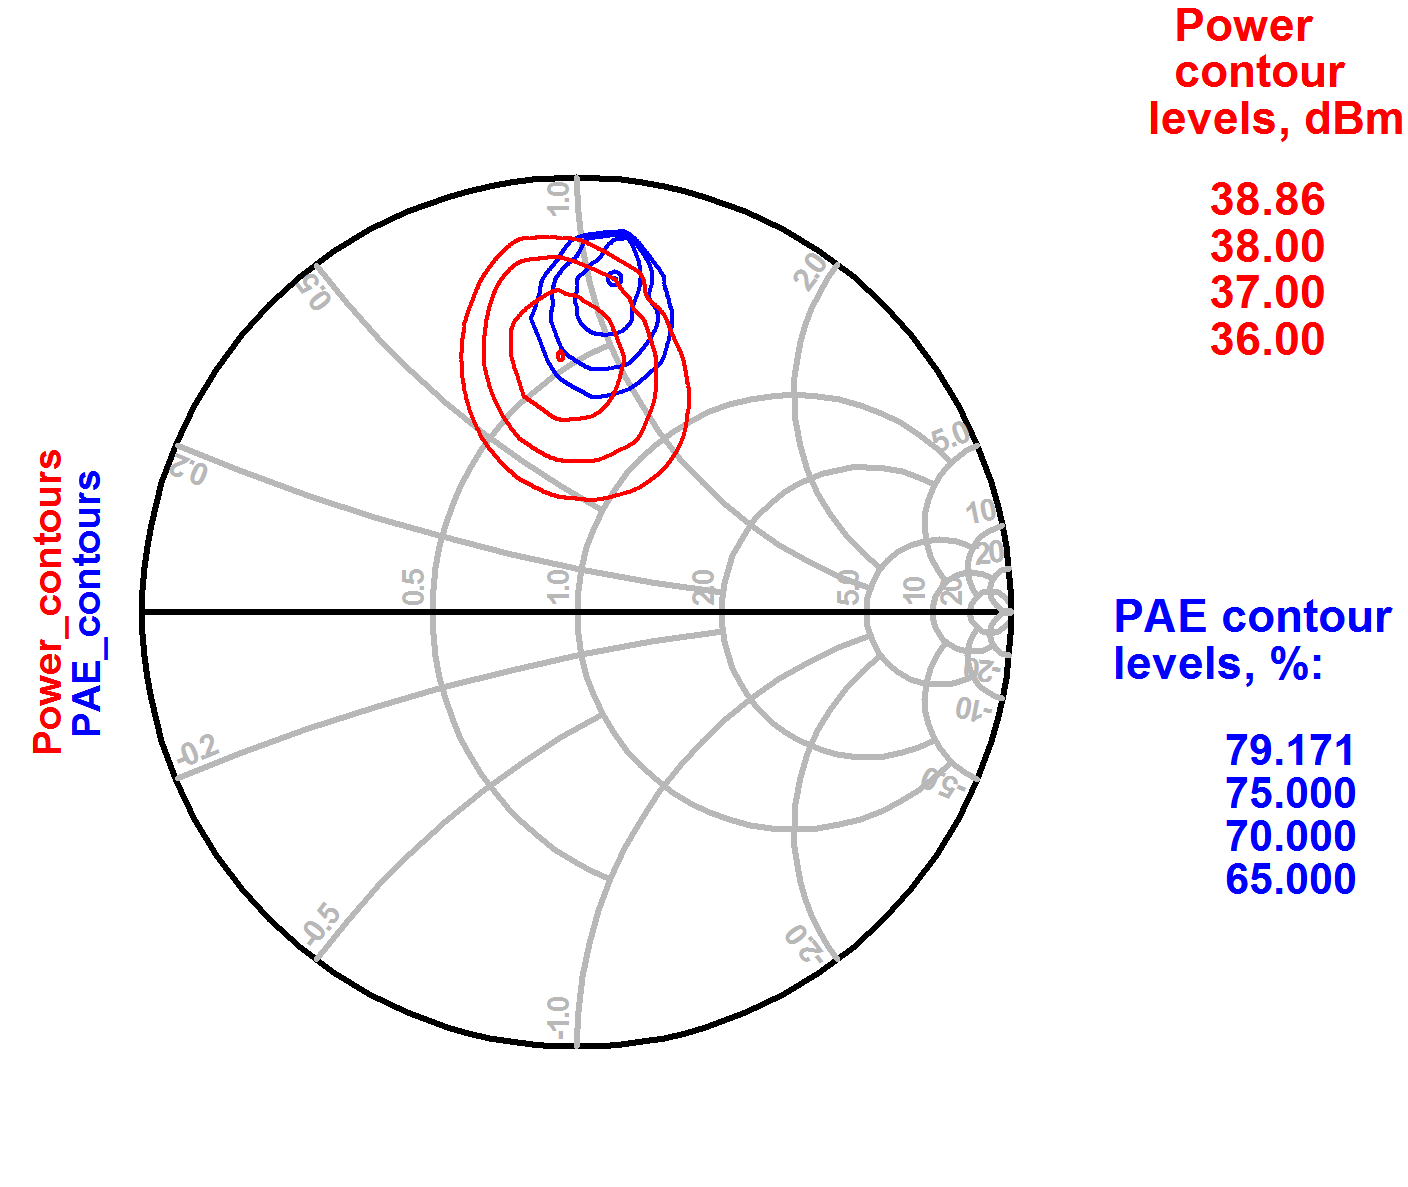
\includegraphics[width=4in,height=4in,keepaspectratio]{figures/simulation/sc_fund_final_load}\\
  \caption{Final Fundamental Load Pull on Smith Chart}
  \label{fig:sc_fund_final_load}

  \vspace*{\floatsep}

  \centering
  % Requires \usepackage{graphicx}
  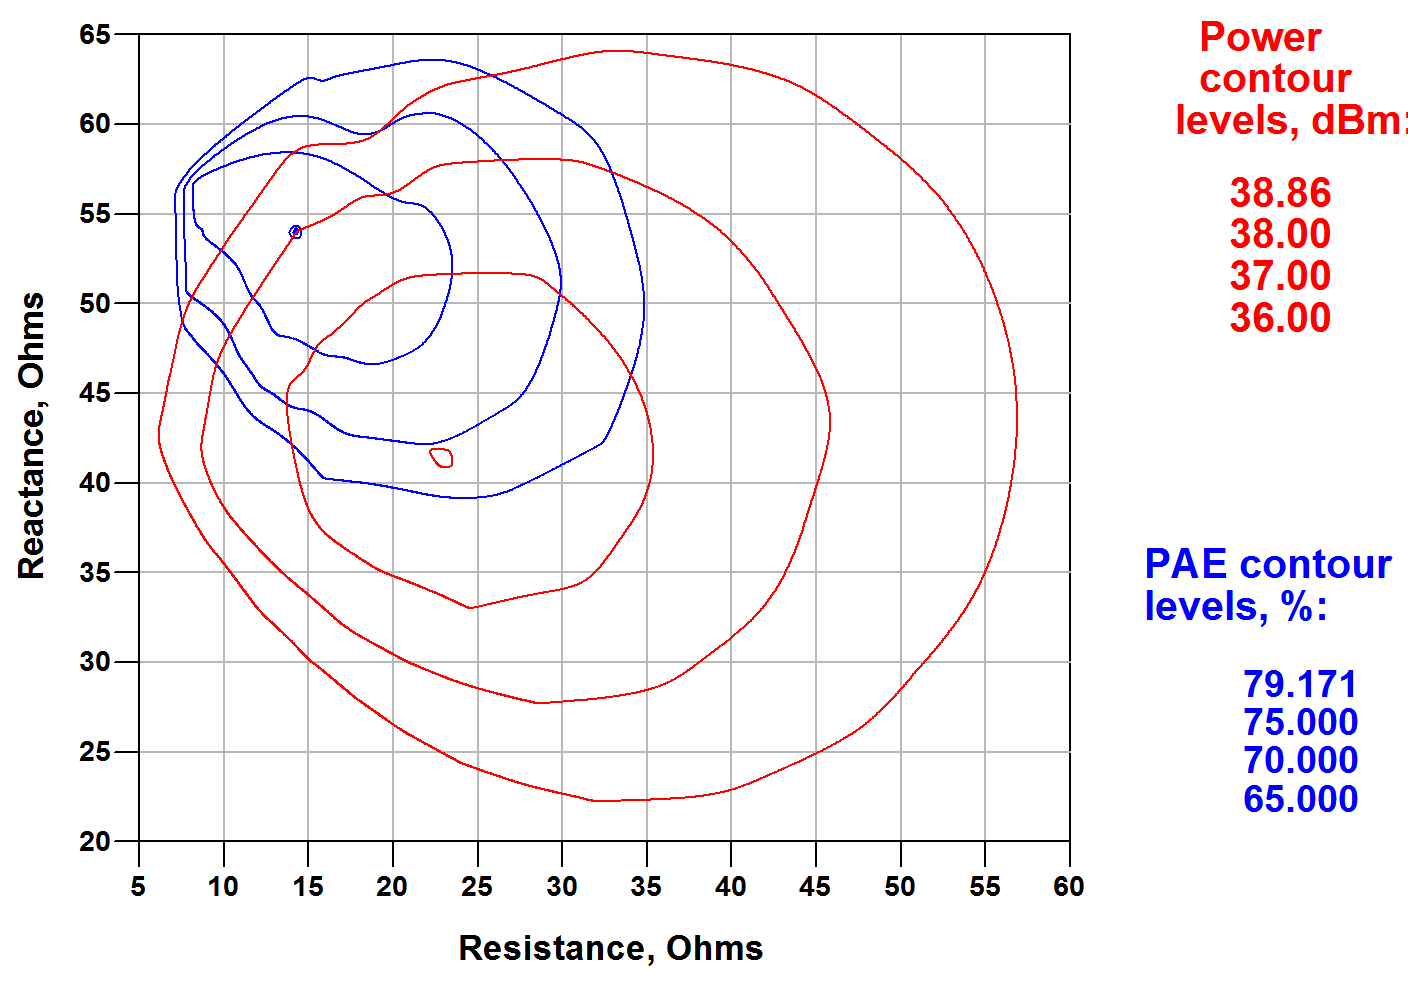
\includegraphics[width=4in,height=4in,keepaspectratio]{figures/simulation/res_cont_fund_load_final}\\
  \caption{Final Fundamental Load Pull Fix This Label}
  \label{fig:res_cont_fund_load_final}
\end{figure}

%%The harmonic phase pull is done at the lowest harmonic from load to source then to the highest harmonic. The harmonic phase pull is done at the input and output because it's been shown experimentally that harmonic matching networks at the input can also increase the drain efficiency INSERT REFERENCE HERE. The harmonic phase pull can measure gain and efficiency contours just like the load and source pulls. The end result of all the various pull simulations is the ideal gain and efficiency of the amplifier in class F operation if the harmonics are ideally terminated. The process of determining a DC bias, fundamental load and source pull, and harmonic phase pulls is repeated until the requirements are met. Table X shows the iteration steps and amplifier performance. Initially the goal was to control up to the fifth harmonic to hopefully increase the efficiency near the theoretical value of 90.5\% CHECK THIS VALUE. But this the transistor used there weren't any sufficient gains from controlling up to the third harmonic versus controlling up to the fifth harmonic so it was decided only up to the third harmonic will be controlled.

%Harmonic phase pull with contours

%Final simulated parameters of transistor

\section{Harmonic matching network}

The harmonic matching network is the key in keeping the proper harmonics at the drain. It is composed of a matching network and a wave shaping network that is on the load and source side of the transistor. The wave shaping network consists of a series section that is a quarter wavelength long with an eight wavelength open shunt stub. An additional series element is added that is used for tuning that goes to a two more stubs that used for the second harmonic and bias circuitry seen in Figure \ref{fig:matching_network_woo}. Most class F wave shaping network follow a similar pattern of various fractional wavelength sections so the drain is properly terminated. The downside of these networks is the relatively large electrical lengths due to the presence of a quarter wavelength sections in nearly all such networks. This design explores if coupling the open circuit shunt stubs in the wave shaping network can decrease the electrical size of the class F amplifier. Two versions of the amplifier were simulated, one that uses coupled microstrip lines and one without to compare the overall electrical size of the amplifier.

%Insert figure of matching network and wave shaping network
\begin{figure}
  \centering
  % Requires \usepackage{graphicx}
  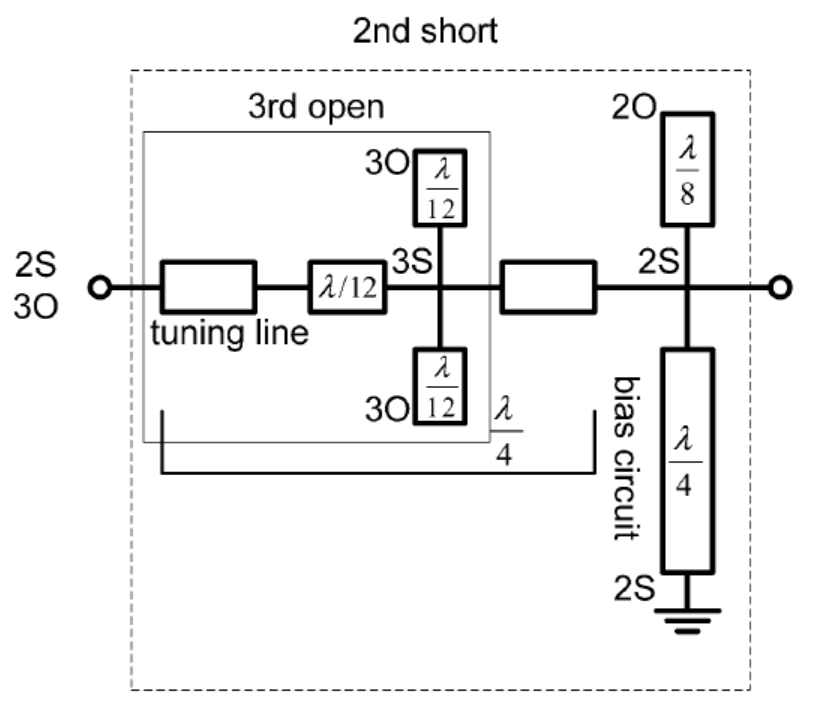
\includegraphics[width=5in,height=5in,keepaspectratio]{figures/simulation/matching_network_woo}\\
  \caption{Matching Network for Amplifier} %cite woo
  \label{fig:matching_network_woo}
\end{figure}

After the wave shaping network comes the matching network so the amplifier is matched as close as possible to 50$\Omega$. This amplifier used a shunt stub and a series transmission line for the matching network on the load and source side.

Need to do two tone tests and stability tests for the amplifier! More content!

\section{Talk about simulated amplifier}
The transmission lines were simulated using Rogers INSERT NUMBER HERE. After comparing various low loss laminates like Duroid, the Rogers NUMBER HERE was selected. This was partially due to the larger sample size that could be ordered so more amplifier boards could be fabricated. Also it has the lowest tangent loss and relative permittivity that allowed the transmission lines going to the transistor gate and drain to be thin enough. Reword all of this later man. All of the amplifier dimensions were set as parameters with goals to maximize the PAE with a minimum set gain at a fixed RF input power and the optimizer was used to tune the amplifier dimensions. The board discussed in this section is the third revision. The previous two amplifiers were malfunctioned with one acting as an oscillator and the other not working at all. This was most likely due to fabrication issues.

The simulated drain current and voltage waveforms can be seen in Figure \ref{fig:ids_vds_wave} which show some partial overlap. Although the waveforms aren't ideal, the amplifier still has high PAE and meets the minimum output power. Even during the off cycle of the drain current, there is still quiescent current flowing which dissipates significant power due to the high drain voltage.

%Drain current and voltage waveforms
\begin{figure}
  \centering
  % Requires \usepackage{graphicx}
  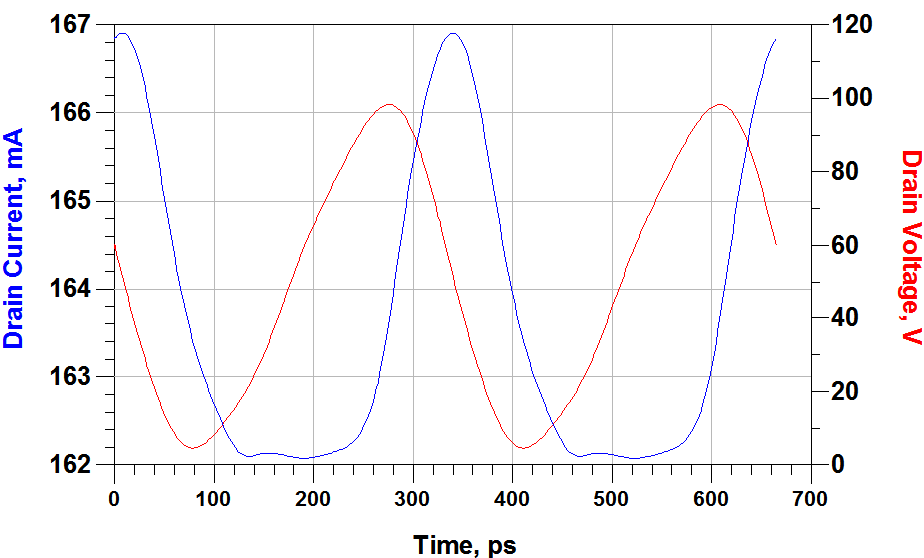
\includegraphics[width=5in,height=5in,keepaspectratio]{figures/simulation/ids_vds_wave}\\
  \caption{Simulated Drain Current and Voltage Versus Time}
  \label{fig:ids_vds_wave}
\end{figure}


%Two tone test
\begin{figure}
  \centering
  % Requires \usepackage{graphicx}
  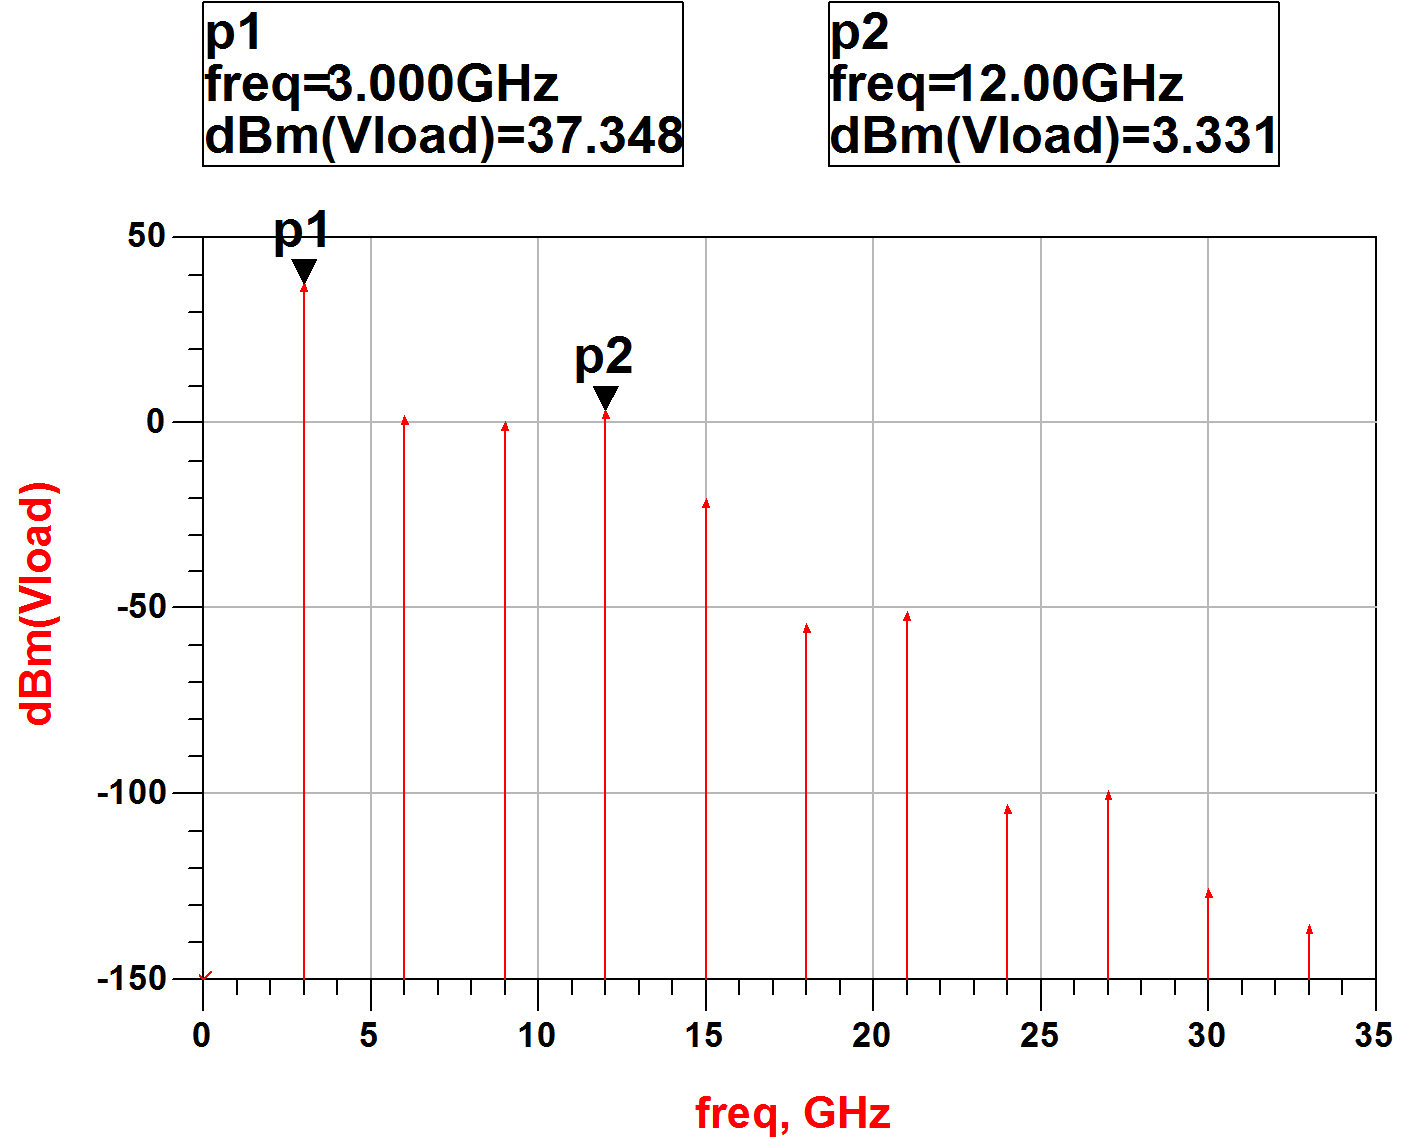
\includegraphics[width=5in,height=5in,keepaspectratio]{figures/amp_sim/IMD_singletone}\\
  \caption{Simulated Single Tone IMD}
  \label{fig:imd_single}

  \vspace*{\floatsep}

  \centering
  % Requires \usepackage{graphicx}
  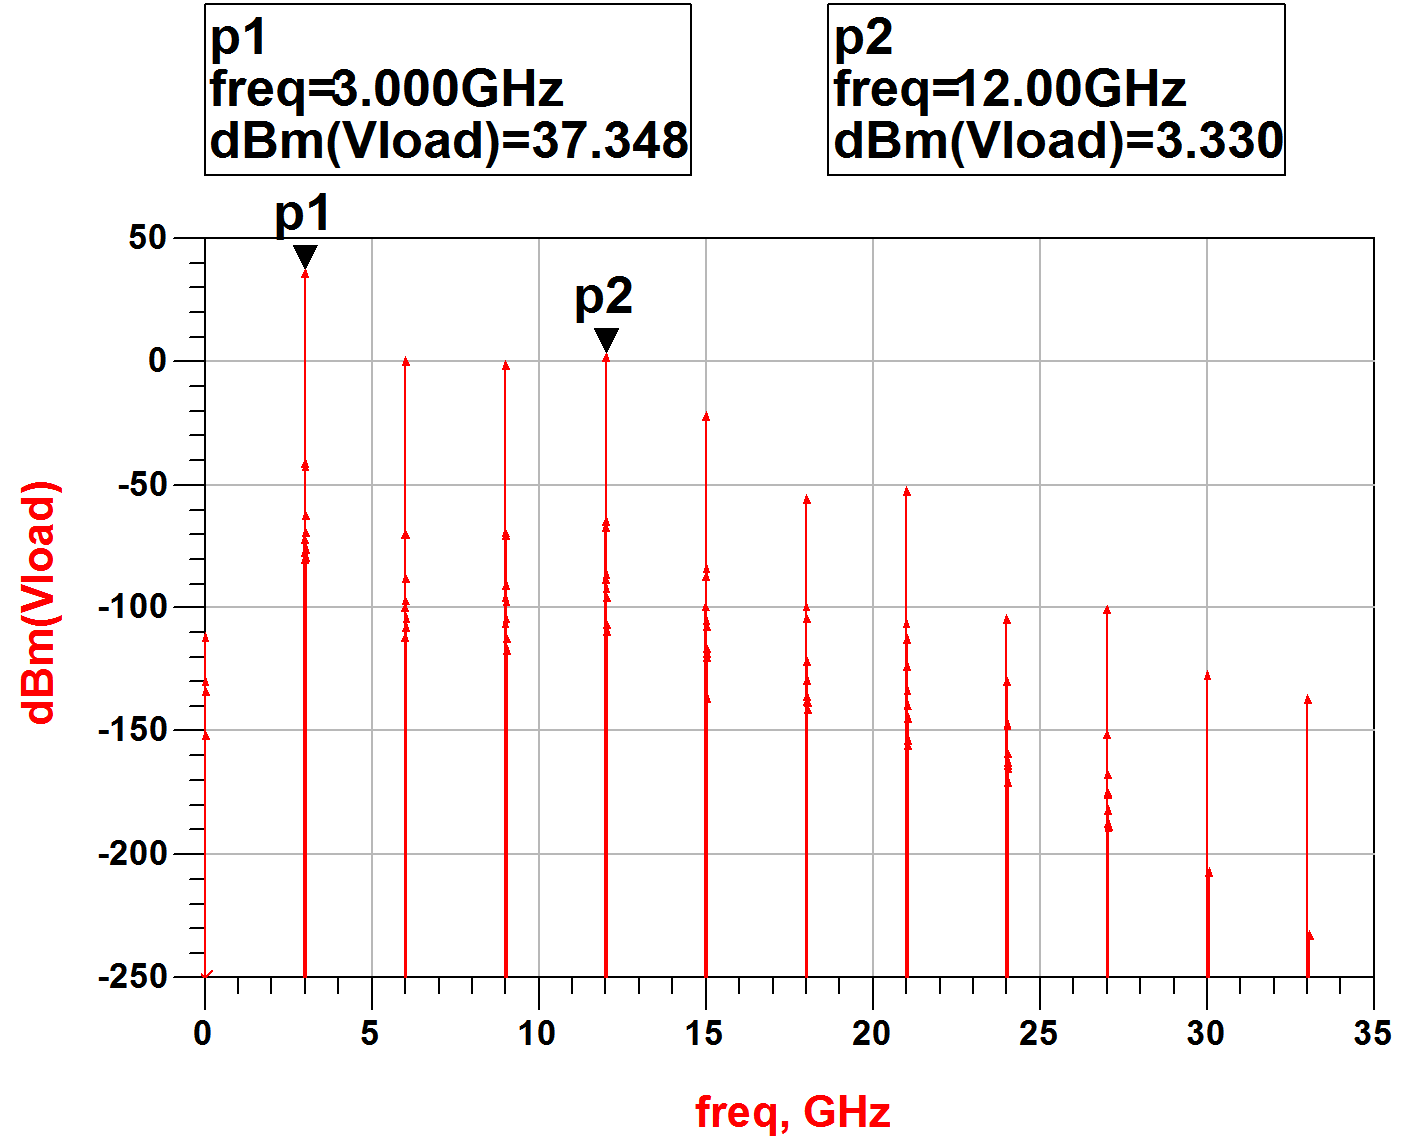
\includegraphics[width=5in,height=5in,keepaspectratio]{figures/amp_sim/IMD_twotone}\\
  \caption{Simulated Two Tone IMD with 10 MHz Offset}
  \label{fig:imd_double}
\end{figure}

VSWR plots
How do get VSWR using harmonic balance?

Gain vs frequency and input power

PAE and Gain vs input power

power out vs power in

Table of simulated amplifier measurements

